\section{Position}
The goal of this project is to create Simpson characters by using LEGO blocks. Therefore, it is imperative to have a precise position of every block in order to give the correct coordinates to the gripper. Thus, the position becomes one of the most important steps in this project.

After detecting the edges of the blocks, it was possible to find the square shapes of the blocks. These shapes were filled up, creating an homogeneous area that allowed a better calculation of the center by using the \textit{'Regionprops'} function. This function calculates the coordinates of the center of mass which will be the center of the selected shape.

\section{Orientation}
Besides the position, the correct angle to turn the gripper is essential in this application. Nevertheless, the coordinates of the center will be important to find the orientation of the blocks. 

Using the image with the edges of only one block, the distance between each point and the center was calculated. Then, the points were sorted in a vector in order to find the coordinates of the four furthest points with respect to the center. However, in some situations a corner can be further from the center than the others, which means that more than one pixel would be selected in the same corner. To avoid this situation, the first pixel in the vector (the furthest one) will be surrounded by a forbidden area in order to choose only one pixel in each vertex (Figure \ref{fig:corner}).

\begin{figure}[H]
\centering
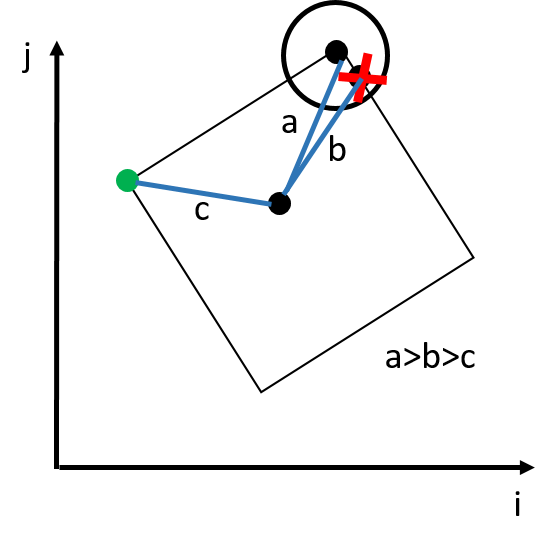
\includegraphics[scale=0.5]{figures/rotation6.png}
\caption{Corner's forbidden area}
\label{fig:corner}
\end{figure}

Then, two of the previous corners are chosen, such that they define one side of the square. The connection between these two corners and the center generates two different straight lines (from each corner to the center). Using the same image, it was evaluated which points were below the generated lines. To finish this step, a linear regression was calculated and the parameters of the straight line were found.

\begin{figure}[H]
\hfill
\subfigure[Straight lines that connect the corners with the center of the block]{

\includegraphics[scale=0.5]{figures/diag_square.png}
\label{fig:subim11}}
\hfill
\subfigure[Side of the square used for calculating the slope]{
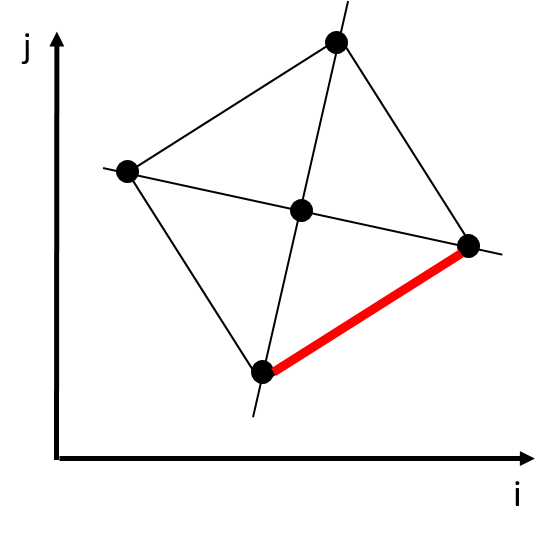
\includegraphics[scale=0.5]{figures/diag_square_side.png}
\label{fig:subim12}}
\hfill
\caption{Block in the world frame}
\end{figure}

Finally, the slope was converted to an angle to obtain the orientation of the block. However, if the angle was negative it was necessary to calculate the one associated with the perpendicular line in order to have the correct orientation.

\begin{figure}[H]
\hfill
\subfigure[Positive slope - it gives directly the orientation]{
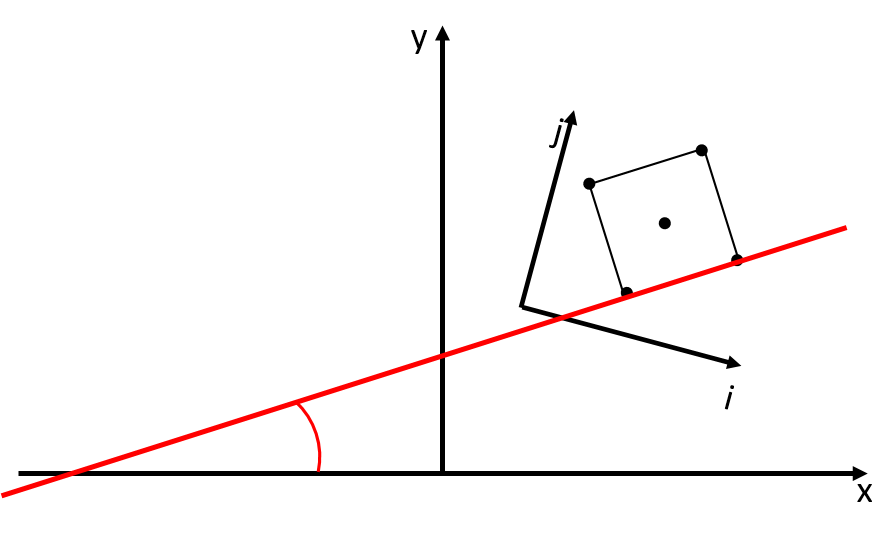
\includegraphics[scale=0.45]{figures/posit_slope.png}
\centering
\label{fig:subim21}}
\hfill
\subfigure[Negative slope - it gives indirectly the orientation]{
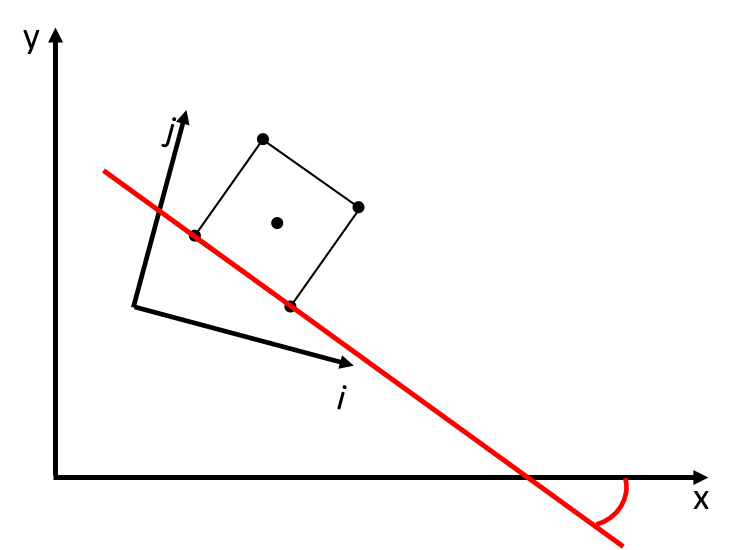
\includegraphics[scale=0.45]{figures/neg_slope.png}
\label{fig:subim22}}
\hfill
\caption{Orientation of the block in the robot frame}
\label{fig:image2}
\end{figure}